\documentclass[12pt,letterpaper,twocolumn]{article}

\usepackage[utf8]{inputenc}
\usepackage[english]{babel}
\usepackage{float}
\usepackage{xcolor}
\usepackage{verbatim}
\usepackage{mwe}
\usepackage{charter}
\usepackage{afterpage}
\usepackage{amsmath}
\usepackage{appendix}
\usepackage{ragged2e}
\usepackage{array}
\usepackage{etoolbox}
\usepackage{fancyhdr}
\usepackage{booktabs}
\usepackage{arydshln}
\usepackage[justification=justified,singlelinecheck=false,labelfont=bf,format=plain]{caption}
\usepackage[justification=justified,singlelinecheck=false,labelfont=bf,format=plain]{subcaption}
\usepackage{enumitem}
\usepackage[bottom=2.5cm,top=2.0cm,left=2.0cm,right=2.0cm]{geometry}
\usepackage{graphicx}
\graphicspath{{img/}}
\usepackage{indentfirst}
\usepackage{mathtools}
\usepackage{multirow}
\usepackage{pdfpages} 
\usepackage{subfiles}
\usepackage[compact]{titlesec}
\usepackage{blindtext}
\usepackage{stfloats}
\usepackage{lipsum} 


\renewcommand{\familydefault}{\rmdefault}

\newcommand\blankpage{
    \null
    \thispagestyle{empty}
    \addtocounter{page}{0}
    \newpage}

\newcolumntype{L}[1]{>{\raggedright\let\newline\\\arraybackslash\hspace{0pt}}m{#1}}
\newcolumntype{C}[1]{>{\centering\let\newline\\\arraybackslash\hspace{0pt}}m{#1}}
\newcolumntype{R}[1]{>{\raggedleft\let\newline\\\arraybackslash\hspace{0pt}}m{#1}}

    \setlist[itemize,1]{label=$\bullet$}
    \setlist[itemize,2]{label=$\circ$}
    \setlist[itemize,3]{label=$-$}
    \setlist{nosep}

\setlength{\columnsep}{30pt}

\titlelabel{\thetitle.\quad}

\pagestyle{fancy}
\fancyhf{}
      
\fancyfoot{}
\fancyfoot[C]{\thepage} % page
\renewcommand{\headrulewidth}{0mm} % headrule width
\renewcommand{\footrulewidth}{0mm} % footrule width

\makeatletter
\patchcmd{\headrule}{\hrule}{\color{black}\hrule}{}{} % headrule
\patchcmd{\footrule}{\hrule}{\color{black}\hrule}{}{} % footrule
\makeatother

\definecolor{blueM}{cmyk}{1.0,0.49,0.0,0.47}

%Bibliography
 \usepackage[
    backend=biber,
    style=bwl-FU,
    sorting=nyt,
  ]{biblatex}
 \addbibresource{references.bib}
 \usepackage{breakcites}

%%%%%%%%%%%%%%%%%%%%%%%%%%%%%%%%%%%%%%%%%%%%%%%%%%%%%%%%%%%%%%%%%%%%%%%%%%%%%%%%%%%%%%%%%%%%%%%%%%%%%%%%%%%%%%%%%%%%%%%%%%%%%%%%%%%%%%%%%%%%%%%%%%%%%%%%%%%%%%%%%%%%%%%%%%%%%%%%%%%%%%%
    
\begin{document}
\twocolumn[\begin{@twocolumnfalse}

\hspace{25pt}
\begin{minipage}{0.75\textwidth}
\vspace{5mm}
    \Large{\textbf{Generalized State-Space Models}} 
    
    \vspace{3mm}
    
    \large{\textbf{Andrea Stragiotti}} \newline
    \fontsize{0.35cm}{0.5cm}\selectfont \textit{MSc in Data Science, UCL\newline}
    \vspace{1mm} 
    
    \today

\end{minipage}

\small

\vspace{11pt}

\centerline{\rule{0.95\textwidth}{0.4pt}}

\begin{center}
    
    \begin{minipage}{0.9\textwidth}
        % ABSTRACT
        \noindent \textbf{Abstract:} 
        
        Generalized state space models are a class of non linear state space models with error distributions that are possibly non normal. In many practical studies the time series considered have measurement not coming from normal distributions, therefore requiring the employment of a generalized approach and a suitable state space. A crucial step in the application of these models is the estimation of the distribution of the variables in the state space to fit the observed state. In this document we will go over the main approaches to the estimation and use of generalized state space models.
    
        \vspace{4mm}
        % KEYWORDS
        \noindent \textbf{Keywords:} State-Space Model
    
    \end{minipage}
    
\end{center}
\centerline{\rule{0.95\textwidth}{0.4pt}}
\vspace{50pt}
\end{@twocolumnfalse}]
%%%%%%%%%%%%%%%%%%%%%%%%%%%%%%%%%%%%%%%%%%%%%%%%%%%%%%%%%%%%
\section{Introduction}
\justify
State space models are dynamic models represented in a well defined state space for easiness of interaction and representation. They have many applications in engineering, economics and other disciplines. 
\par \vspace{5mm}
A state space models is defined as:
\begin{equation} \label{eq:measure}
    Y_t = \textbf{B}^T \textbf{S}_t + \epsilon_t
\end{equation}
\begin{equation} \label{eq:trans}
    \textbf{S}_t =  \textbf{C}\textbf{S}_{t-1} + \textbf{H}_t
\end{equation}
With the covariance matrix of \textbf{H} being \textbf{V}.
\par \vspace{5mm}
One of the main assumptions on state space models to make tractability of the model easier is to assume normality of the distribution of the error terms both in the measurement or observation equation (\ref{eq:measure}) and the transition or state equation (\ref{eq:trans}).
\par \vspace{5mm}
One of the most useful features of state space models is the Kalman filter (\cite{kalman1960}). While the intuition behind the filter doesn't rely on the normality of the data, the ability to compute multiple steps ahead of the model is grounded on normality to make the necessary simplifications.
\par \vspace{5mm}
The Kalman filter is a recursive procedure for calculating the optimal estimator of the state vector $\textbf{S}_t$ given all the information available. The procedure relies on the previously defined variables and on \textbf{P}, the covariance matrix of the associated estimation error:
\begin{equation}
    \textbf{P}_{t|t-k} = E((\textbf{S}_t - \widehat{\textbf{S}}_{t|t-k})^T(\textbf{S}_t - \widehat{\textbf{S}}_{t|t-k}))
\end{equation}
Having defined those quantities the Kalman filter procedure would consist of the following equations:
\begin{equation}
  \label{eq:kalman}
  \begin{gathered}
    \widehat{\textbf{S}}_{t|t-1} = \textbf{C}\widehat{\textbf{S}}_{t-1|t-1}\\
    \textbf{P}_{t|t-1} =  \textbf{C}\textbf{P}_{t-1|t-1}\textbf{C}^T + \textbf{V}\\
    f_t = \textbf{B}^T\textbf{P}_{t|t-1}\textbf{B} + \sigma^2\\
    \widehat{\textbf{S}}_{t|t} = \widehat{\textbf{S}}_{t|t-1} + \textbf{P}_{t|t-1}
    \textbf{B}(Y_t - \textbf{B}^T\widehat{\textbf{S}}_{t|t-1})/f_t\\
    \textbf{P}_{t|t} =  \textbf{P}_{t|t-1} -  \textbf{P}_{t|t-1}\textbf{B}\textbf{B}^T \textbf{P}_{t|t-1} /f_t
  \end{gathered}
\end{equation}
Where \textbf{C} is the transition matrix between hidden states, $f_t$ is the adjustment factor which is part of the Kalman Gain. $f_t$ might also be interpreted as the the variance of the prediction error $Y_t - \hat{Y_t}$.
\par \vspace{5mm}
Generalized State Space Models (GSSM) do not rely on the previous assumptions of normality and are therefore suitable for different types of analysis with non-normally distributed data.

The main difference in GSSM from the previous introduction is in the two equations (\ref{eq:measure}) and (\ref{eq:trans}). In there we need to define the measurement equation:
\begin{equation} \label{eq:gener_measure}
    Y_t|\textbf{S}_t \sim f_t(y|\textbf{S}_t) dy 
\end{equation}
And the transition equation:
\begin{equation} \label{eq:gener_trans}
    \textbf{S}_t|\textbf{S}_{t-1} \sim g_t(\textbf{S}|\textbf{S}_t) d\textbf{S}_t
\end{equation}
This generalized state space model will be governed by the conditional densities $f_t$ and $g_t$ defined there. Obviously the generalization of a Kalman filter approach to the GSSM requires a higher degree of complexity and possibly some approximations.

We will now review the literature around the two distributions and how they have been approached and approximated through time.

\section{Literature Review}
\justify
Generalized State Space Models are flexible and suitable for a variety of time series data. We can find various examples of applications of such models in literature. We present some of the work on GSSM below, with a focus on the initial generalization of normal approaches and the first applications of them.
\par \vspace{5mm}
In (\cite{kitagawa1987}) an approach to generalized state space models is presented and applied to a real data-set. This is the first introduction of a technique implying non normality in the noise processes of the state space. In his paper Kitagawa allows for $\epsilon$ and \textbf{V} to be non normal. Numerous attempts to include non normality in state space models are then covered but only the method proposed in the paper deals with it directly instead of forcing some kind of transformation to the data. The author proposes to estimate an approximation of the density function and uses a spline to approximate it. With a sufficiently small interval the density function can be reasonably estimated and therefore used to update the one step ahead prediction of the model.
\par \vspace{5mm}
In (\cite{song2007correlated}) a frequentist approach and a Bayesian approach to GSSM are presented. The model presented in the introduction had no assumptions made while the Kalman filter equations \eqref{eq:kalman} relied on the assumption of normality to update the matrix \textbf{P} of probabilities distribution. In a generalized case this is not possible and in the book the authors propose different approaches as to how to estimates such quantities in the filter. \textbf{P} is therefore defined as:
\begin{equation}
    \label{eq:distprob}
    \textbf{P}_{t|t-1} = \int{\textbf{P}_{t-1|t-1}g_t(\textbf{S}_t|\textbf{S}_{t-1})
    d\textbf{S}_{t-1}}
\end{equation}
where $g_t$ is the distribution probability of the state matrix \textbf{S} conditional on the previous state of the model. This cannot be further simplified since we cannot make assumptions on $g$. From here the authors propose several approaches to the estimation of the integral. The Bayesian approach is making use of the Monte Carlo method which is effectively approximating the probability density of $\textbf{S}_t$ as:
\begin{equation}
    \textbf{S}_t = \frac{1}{M}\sum_{i=1}^{M} \textbf{S}_t^{(i)}
\end{equation}
Where $\textbf{S}^i$ is the sampled state from the original observed data \textbf{Y}.
\par \vspace{5mm}
In (\cite{jorgsong98}) the authors focus on count longitudinal data, using Poisson distributions to approximate the density function of the state space model. The main contribution from the paper is the use of an approximation function instead of a Monte Carlo approach to estimate the distribution $g$. The approximation function is part of the Tweedie class which has the following density form:
\begin{equation}
    f(y: \mu, \sigma^2, p) = c_p(y: \sigma^2)e^{\frac{1}{\sigma^2}(y\tau_p^{-1}(\mu) - \kappa{\tau_p^{-1}(\mu)})}
\end{equation}
Where $\mu$ is the mean parameter, $\sigma^2$ the dispersion parameter and $p$ the shape parameter.
Such a distribution allows the Kalman filter equation to be derived analytically as demonstrated in the technical appendix of the paper.

\section{Examples}
\justify
The use of generalized state space models has multiple applications. In (\cite{song2007correlated}) several applications are presented.

\subsection{Generalized State Space Models for Longitudinal Binomial Data}
In some cases the data analysed in a time series are not observations extrapolated from a normal distribution but a binomial one, i.e. the presence or absence of a specific state.

In (\cite{kitagawa1987}) the Tokyo Rainfall Data is presented. The data is presenting the number of occurrences of rainfall over 1 mm in Tokyo as a proxy of a rainy versus non-rainy day. This is of course a type of non normal data and therefore might be modeled using a GSSM. In this case the use of a binomial distribution seems the best approach.
\par \vspace{5mm}
The equations governing the model are:
\begin{equation}
    \begin{gathered}
        Y_t|S_t \sim Bi(2, \pi_t) \text{ with } \pi_t = \sigma(S_t)\\
        S_t = S_{t-1} + \epsilon_t
    \end{gathered}
\end{equation}
The state process is therefore assumed to be a random walk. With these definitions the predicted time series using a Kalman predictor would be the following.

\begin{figure}
    \centering
    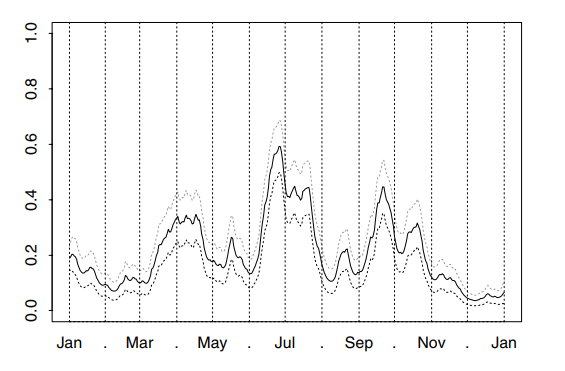
\includegraphics[width=8.5cm]{tokyo_rainfall.PNG}
    \caption{Monte Carlo predicted probability process based on the Kalman smoother proposed above}
    \label{fig:rain}
\end{figure}

The figure (\ref{fig:rain}) clearly indicates some kind of seasonal pattern over the year in Tokyo. The summer season seems to be the wettest for the city while winter is usually dry. The approach is fairly simple, but it relies on an additional step on top of what we already highlighted in the literature review (Equation \eqref{eq:distprob}). Once \textbf{P} is defined also the rest of the Kalman filter generalized quantities needs to be derived. This is:
\begin{equation}
    \textbf{P}_{t|t} = g_t(\textbf{S}_{t|t-1})\textbf{P}_{t|t-1}/\textbf{B}^t\textbf{P}_{t|t-1}\textbf{B}+\sigma^2
\end{equation}
As derived in (\cite{kitagawa1987} - Equation 2.3). From there, recursively applying the equations leads us to the discussed data.

\subsection{Generalized State Space Models for Longitudinal Count Data}

In some other cases the time series is related to count data. Again we cannot assume normality in such a case and we need GSSM to model the data.

In (\cite{Scot-1988}) we are presented with a count time series of poliomyelitis disease incidence over the US population between 1970 and 1983. We also observe the exposure to environments that might increase the risk of contracting the disease. In this case the measurement equation might take the form:
\begin{equation}
    Y_t|S_t \sim Po(a_t, S_t) \text{ with } a_t = e^{x_t^T\alpha}
\end{equation}
where 
\begin{equation}
\begin{gathered}
    x_t = (1, t, cos(2\pi t/12), sin(2\pi t/12), \\
    cos(2\pi t/6), sin(2\pi t/6))
    \end{gathered}
\end{equation}
In a similar fashion to what we discussed above, the authors of the paper derive a Kalman filter and smoother equations system to model the incidence of the data.

\begin{figure}
    \centering
    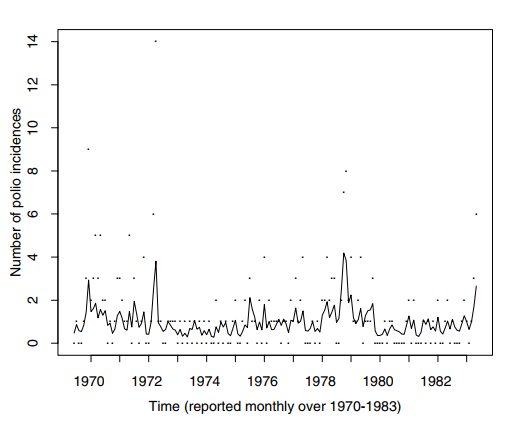
\includegraphics[width=8.5cm]{polio.PNG}
    \caption{Predicted probability process based on the Kalman smoother for the polio data. Dot shows observed counts and the solid line present the estimated process}
    \label{fig:polio}
\end{figure}

The  result is reassuring: the trend in the data is significantly different from zero and negative, showing a reduced impact of the disease on the population over time.

\section{Conclusion}
\justify

While the use of normal state space models is widespread and well understood, the use of non linear methods requires further work. We presented the theory behind generalized state space models and we reviewed some of the main applications for binomial and count data. The main approach to these methods relies on Monte Carlo methods and it's therefore highly dependent on the computational power offered to approach the problem. The increase in computational power and estimation techniques suggest a strong case for the employment of such models when the data is non normal.

\printbibliography

\end{document}
